%%%%%%%%%%%%%%%%%%%%%%%%%%%%%%%%%%%%%%%%%
% Masters/Doctoral Thesis 
% LaTeX Template
% Version 2.4 (22/11/16)
%
% This template has been downloaded from:
% http://www.LaTeXTemplates.com
%
% Version 2.x major modifications by:
% Vel (vel@latextemplates.com)
%
% This template is based on a template by:
% Steve Gunn (http://users.ecs.soton.ac.uk/srg/softwaretools/document/templates/)
% Sunil Patel (http://www.sunilpatel.co.uk/thesis-template/)
%
% Template license:
% CC BY-NC-SA 3.0 (http://creativecommons.org/licenses/by-nc-sa/3.0/)
%
%%%%%%%%%%%%%%%%%%%%%%%%%%%%%%%%%%%%%%%%%

%----------------------------------------------------------------------------------------
%	PACKAGES AND OTHER DOCUMENT CONFIGURATIONS
%----------------------------------------------------------------------------------------

\documentclass[
11pt, % The default document font size, options: 10pt, 11pt, 12pt
%oneside, % Two side (alternating margins) for binding by default, uncomment to switch to one side
english, % ngerman for German
singlespacing, % Single line spacing, alternatives: onehalfspacing or doublespacing
%draft, % Uncomment to enable draft mode (no pictures, no links, overfull hboxes indicated)
%nolistspacing, % If the document is onehalfspacing or doublespacing, uncomment this to set spacing in lists to single
%liststotoc, % Uncomment to add the list of figures/tables/etc to the table of contents
%toctotoc, % Uncomment to add the main table of contents to the table of contents
%parskip, % Uncomment to add space between paragraphs
%nohyperref, % Uncomment to not load the hyperref package
headsepline, % Uncomment to get a line under the header
%chapterinoneline, % Uncomment to place the chapter title next to the number on one line
%consistentlayout, % Uncomment to change the layout of the declaration, abstract and acknowledgements pages to match the default layout
]{MastersDoctoralThesis} % The class file specifying the document structure

\usepackage[utf8]{inputenc} % Required for inputting international characters
\usepackage[T1]{fontenc} % Output font encoding for international characters

\usepackage{palatino} % Use the Palatino font by default

\usepackage[backend=bibtex,style=authoryear,natbib=true]{biblatex} % Use the bibtex backend with the authoryear citation style (which resembles APA)

\addbibresource{example.bib} % The filename of the bibliography

\usepackage[autostyle=true]{csquotes} % Required to generate language-dependent quotes in the bibliography

\usepackage{listings}

\addto\captionsenglish{%
  \renewcommand{\chaptername}{Capítulo}
  \renewcommand{\contentsname}{Índice General}%Table of contents
  \renewcommand{\listfigurename}{Índice de Figuras}    %Figures
  \renewcommand{\listtablename}{Índice de Tablas}        %Tables
  \renewcommand{\figurename}{Figura}              %Figure
  \renewcommand{\tablename}{Tabla}                %Table
  %\renewcommand{\bibname}{Bibliografía}             %Bibliography REferencias refname
   %\renewcommand{\refname}{Bibliografía}             %Bibliography REferencias refname
 \renewcommand{\lstlistingname}{Código}% Listing -> Algorithm
\renewcommand{\lstlistlistingname}{List of Códigos}
 \renewcommand{\appendixname}{Apéndice}   %Appendix
}

%----------------------------------------------------------------------------------------
%	MARGIN SETTINGS
%----------------------------------------------------------------------------------------

\geometry{
	paper=a4paper, % Change to letterpaper for US letter
	inner=2.5cm, % Inner margin
	outer=3.8cm, % Outer margin
	bindingoffset=.5cm, % Binding offset
	top=1.5cm, % Top margin
	bottom=1.5cm, % Bottom margin
	%showframe, % Uncomment to show how the type block is set on the page
}

%----------------------------------------------------------------------------------------
%	THESIS INFORMATION
%----------------------------------------------------------------------------------------

\thesistitle{\textsc{Procesamiento de voz para mejorar la pronunciación}} % Your thesis title, this is used in the title and abstract, print it elsewhere with \ttitle
\supervisor{} % Your supervisor's name, this is used in the title page, print it elsewhere with \supname
\examiner{} % Your examiner's name, this is not currently used anywhere in the template, print it elsewhere with \examname
\degree{Doble grado en Ingeniería Informática y Matemáticas} % Your degree name, this is used in the title page and abstract, print it elsewhere with \degreename
\author{Mayra Alexandra Castrosqui Florián} % Your name, this is used in the title page and abstract, print it elsewhere with \authorname
\addresses{} % Your address, this is not currently used anywhere in the template, print it elsewhere with \addressname

\subject{Trabajo de Fin de Grado} % Your subject area, this is not currently used anywhere in the template, print it elsewhere with \subjectname
\keywords{Procesamiento de señales, detección de blobs} % Keywords for your thesis, this is not currently used anywhere in the template, print it elsewhere with \keywordnames
\university{\href{http://www.ucm.es}{Universidad Complutense de Madrid}} % Your university's name and URL, this is used in the title page and abstract, print it elsewhere with \univname
\department{\href{http://department.university.com}{Departamento de Sistemas Informáticos y Computación}} % Your department's name and URL, this is used in the title page and abstract, print it elsewhere with \deptname
\group{\href{http://researchgroup.university.com}{no group}} % Your research group's name and URL, this is used in the title page, print it elsewhere with \groupname
\faculty{\href{http://informatica.ucm.es}{Facultad de Informática}} % Your faculty's name and URL, this is used in the title page and abstract, print it elsewhere with \facname

\AtBeginDocument{
\hypersetup{pdftitle=\ttitle} % Set the PDF's title to your title
\hypersetup{pdfauthor=\authorname} % Set the PDF's author to your name
\hypersetup{pdfkeywords=\keywordnames} % Set the PDF's keywords to your keywords
%\hypersetup{allcolors=blue}
%\hypersetup{urlcolor=blue}
%\hypersetup{citecolor=green}

%\hypersetup{colorlinks=false} % obvious links in the PDF but not the printed text,
}

\begin{document}

\frontmatter % Use roman page numbering style (i, ii, iii, iv...) for the pre-content pages

\pagestyle{plain} % Default to the plain heading style until the thesis style is called for the body content

%----------------------------------------------------------------------------------------
%	TITLE PAGE
%----------------------------------------------------------------------------------------

\begin{titlepage}
\begin{center}

\HRule \\[0.4cm] % Horizontal line
{\huge \bfseries \ttitle\par}\vspace{0.4cm} % Thesis title
\HRule \\[1.5cm] % Horizontal line

\LARGE \authorname \\[0.5cm]
\textsc{\Large \degreename}\\ %  degree
\textsc{\Large \facname}\\ %  faculty
\textsc{\Large \univname}\\[1.5cm] % university

%
\includegraphics[width=6cm]{Figures/TFZsuperellipse_bw} \\[1.5cm] % logo

\includegraphics[width=6cm]{Figures/UCM} \\[1.5cm] % logo


\textsc{\LARGE \subjectname}\\ % TFG
\Large Febrero 2017 \\[1.5cm] 

\large \emph{Director:} Adrián Riesco \\
\large \emph{Codirector:} Enrique Martín Martín \\
 
\vfill
\end{center}
\end{titlepage}

%----------------------------------------------------------------------------------------
%	DECLARATION PAGE
%----------------------------------------------------------------------------------------


%----------------------------------------------------------------------------------------
%	QUOTATION PAGE
%----------------------------------------------------------------------------------------

\vspace*{0.2\textheight}

\noindent\enquote{\itshape quote}\bigbreak

\hfill author

%----------------------------------------------------------------------------------------
%	ABSTRACT - ESPAÑOL
%----------------------------------------------------------------------------------------

%\begin{abstract} % NO USAR PLANTILLA
%\addchaptertocentry{\abstractname} % Add the abstract to the table of contents
%\end{abstract}

\addchaptertocentry{Resumen} % Add the abstract to the table of contents
\addchap*{Resumen}%

Under construction Under construction Under construction Under construction Under construction
Under construction Under construction Under construction Under construction Under construction
Under construction Under construction Under construction Under construction Under construction 
\\

Keywords: \keywordnames, \ldots

%----------------------------------------------------------------------------------------
%	ABSTRACT - ENGLISH
%----------------------------------------------------------------------------------------

%\begin{abstract} % NO USAR PLANTILLA
%\addchaptertocentry{\abstractname} % Add the abstract to the table of contents
%\end{abstract}

\addchaptertocentry{Abstract} % Add the abstract to the table of contents
\addchap*{Abstract}%

Under construction Under construction Under construction Under construction Under construction
Under construction Under construction Under construction Under construction Under construction
Under construction Under construction Under construction Under construction Under construction 
\\

Keywords: \keywordnames, \ldots % en inglés!


%----------------------------------------------------------------------------------------
%	ACKNOWLEDGEMENTS
%----------------------------------------------------------------------------------------

\begin{acknowledgements} % NO USAR PLANTILLA
\addchaptertocentry{\acknowledgementname} % Add the acknowledgements to the table of contents
Under construction %The acknowledgments and the people to thank go here, don't forget to include your project advisor\ldots
\end{acknowledgements}

%----------------------------------------------------------------------------------------
%	LIST OF CONTENTS/FIGURES/TABLES PAGES
%----------------------------------------------------------------------------------------

\tableofcontents % Prints the main table of contents

\listoffigures % Prints the list of figures

\listoftables % Prints the list of tables

%----------------------------------------------------------------------------------------
%	ABBREVIATIONS
%----------------------------------------------------------------------------------------

%\begin{abbreviations}{ll} % Include a list of abbreviations (a table of two columns)
\addchap*{Lista de Abreviaturas}%
%\addchaptertocentry{Lista de Abreviaturas} %add to table of contents?
\begin{longtable}{ll}
\textbf{DSP} & \textbf{D}igital \textbf{S}ignal \textbf{P}rocessing\\
\textbf{FIR} & \textbf{F}inite \textbf{I}mpulse \textbf{R}esponse\\
\textbf{IIR} & \textbf{I}nfinite \textbf{I}mpulse \textbf{R}esponse\\
\end{longtable}
\addtocounter{table}{-1} % Don't count this table as one of the document tables
%\end{abbreviations}

%----------------------------------------------------------------------------------------
%	PHYSICAL CONSTANTS/OTHER DEFINITIONS
%----------------------------------------------------------------------------------------


%----------------------------------------------------------------------------------------
%	SYMBOLS
%----------------------------------------------------------------------------------------


%----------------------------------------------------------------------------------------
%	DEDICATION
%----------------------------------------------------------------------------------------

%\dedicatory{For/Dedicated to/To my\ldots nobody} 

%----------------------------------------------------------------------------------------
%	THESIS CONTENT - CHAPTERS
%----------------------------------------------------------------------------------------

\mainmatter % Begin numeric (1,2,3...) page numbering

\pagestyle{thesis} % Return the page headers back to the "thesis" style

% Include the chapters of the thesis as separate files from the Chapters folder
% Uncomment the lines as you write the chapters

% Chapter Template

\chapter{Introducción} % Main chapter title

\label{Chapter1} % Change X to a consecutive number; for referencing this chapter elsewhere, use \ref{ChapterX}

%----------------------------------------------------------------------------------------
%	SECTION 1
%----------------------------------------------------------------------------------------

\section{Motivación}

Section UNDER CONSTRUCTION Lorem ipsum dolor sit amet, consectetur adipiscing elit.\cite{REF}

%-----------------------------------
%	SUBSECTION 1
%-----------------------------------
\subsection{Subsection 1}

Subsection UNDER CONSTRUCTION posuere quam at lectus tristique eu ultrices augue venenatis. Vestibulum ante ipsum primis in faucibus orci luctus et ultrices posuere cubilia Curae.


%----------------------------------------------------------------------------------------
%	SECTION 2
%----------------------------------------------------------------------------------------

\section{Objetivos}

Section UNDER CONSTRUCTION Sed ullamcorper quam eu nisl interdum at interdum enim egestas. Aliquam placerat justo sed lectus lobortis ut porta nisl porttitor.

%----------------------------------------------------------------------------------------
%	SECTION 3
%----------------------------------------------------------------------------------------

\section{Fundamentos}

Section UNDER CONSTRUCTION Wosuere quam at lectus tristique eu ultrices augue venenatis. Vestibulum ante ipsum primis in faucibus orci luctus et ultrices posuere cubilia Curae

%----------------------------------------------------------------------------------------
%	SECTION 4
%----------------------------------------------------------------------------------------

\section{Estructura de la memoria}

Section UNDER CONSTRUCTION Fosuere quam at lectus tristique eu ultrices augue venenatis. Vestibulum ante ipsum primis in faucibus orci luctus et ultrices posuere cubilia Curae


%!TEX root = ../main.tex

\chapter{Diseño e implementación} % Main chapter title

\label{Chapter2} % for referencing this chapter elsewhere, use \ref{ChapterX}

En esta sección explicaremos detenidamente los distintos pasos que se llevaron a cabo para obtener la aplicación final. \\

Como se ha indicado en la introducción, la tarea fundamental de nuestra aplicación consiste en procesar lo que diga el usuario para poder comparar su pronunciación con la de un nativo. La aplicación está enfocada al tratamiento y comparación del sonido y puede ser incluida por cualquier otra aplicación con interfaz de usuario, ya sea una aplicación móvil, de escritorio u online. Teniendo esto en cuenta se diseñó la aplicación.\\

Una de las decisiones fue programar en lenguaje Java ya que es con el que tengo más dominio y experiencia. \todo{REVISAR porque tiene que tener sentido con que al principio era android } % REVISAR
Además, Java tiene muchas bibliotecas y recursos que hemos tratado de aprovechar. El código puede encontrarse REF \cite{REF} % REF
 y es código abierto y libre. La estructura del código de la aplicación se puede encontrar en esta memoria. REF \cite{REF} \\ % REF

Daremos en primer lugar una visión general de todo el programa. Cuando una persona use el programa se grabará diciendo una frase indicada y la aplicación dirá si la pronunciación ha sido suficientemente buena y leal a la de un nativo. Por ello, el primer paso es obtener un audio directamente del micrófono del medio que esté usando el usuario. El sonido capturado se guardará digitalmente como una secuencia de intensidades que contienen toda la información de audio, este contiene muchas frecuencias no útiles para nuestro objetivo de comparar voces pronunciando la misma frase. Por ello habrá una etapa de filtrado. Después se hará una transformación de Fourier a la señal dividida en segmentos, que nos dará el valor de los impulsos por frecuencia de los segmentos. Aprovecharemos que se encuentra en el dominio de la frecuencia para quitar el sonido de fondo. Y con el espectrograma resultante de la transformación limpia nos quedaremos con la matriz bidimensional asociada, donde cada valor representa la intensidad del impulso por tiempo (segmento) y frecuencia. Esta matriz se puede interpretar como una imagen donde el color en cada punto se consigue a partir del elemento correspondiente en la matriz. Una vez que tenemos la imagen, se hace una detección de blobs o regiones para distinguir las zonas más destacables o sobresalientes de la imagen. Con esto conseguiremos una matriz de valores con más contraste y lista para ser comparada con otra matriz de la misma clase, teniendo en cuenta que las dimensiones de las matrices pueden variar ya sea por la velocidad o volumen del hablante.\\

En el resto de la sección daremos los detalles de estos pasos, dando en primer lugar una explicación teórica y desarrollando después los principales aspectos de implementación.

%----------------------------------------------------------------------------------------
%	SECTION 1
%----------------------------------------------------------------------------------------

\section{Capturando la voz}

Cuando el usuario grabe su voz para ser procesada debemos capturar el audio en un formato que nos facilite su tratamiento. Grabar en formato de audio \emph{raw} nos da total control y visualización de los datos capturados.
Cuando emitimos el sonido para ser grabado emitimos una señal analógica (continua) que el micrófono captura y guarda en forma de señal digital (discreta). 
La transformación de esta señal analógica a digital se hace a través de un proceso llamado muestreo.
En procesamiento de señales, el muestreo es la reducción de una señal continua a una señal discreta. Consiste en tomar muestras de una señal analógica a una frecuencia o tasa de muestreo (\emph{sample rate}) constante, para cuantificarlas y codificarlas posteriormente. La cuantificación consiste en atribuir un valor finito (discreto) de amplitud a cada muestra, un valor dentro de un conjunto específico de valores que luego es codificado en bits.\\

En la figura \ref{fig:sampling} podemos observar cómo se toman muestras discretas $S_i$ de la señal continua $S(t)$ cada $T$ unidades de tiempo.

\begin{figure}[th]
\centering
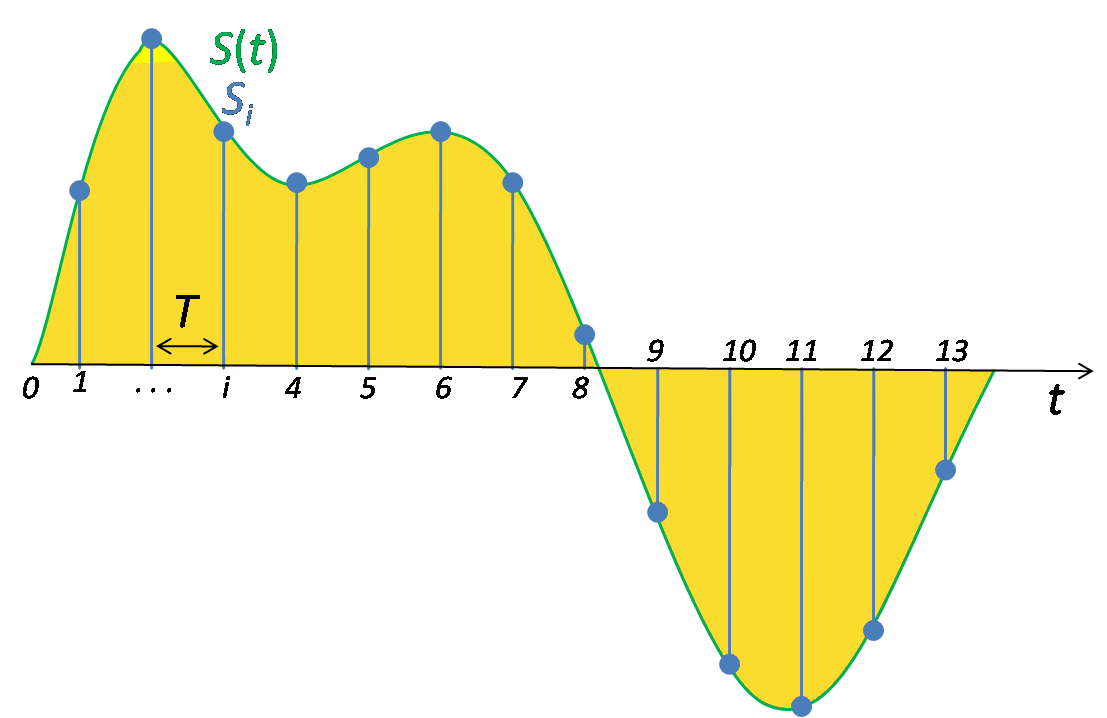
\includegraphics[width=7cm]{Figures/Signal_Sampling}
\decoRule
\caption[Muestreo]{Muestreo de una señal continua para obtener una señal discreta.}
\label{fig:sampling}
\end{figure}

Por tanto, el sonido se graba en muestras discretas y la velocidad con la que se toman estas muestras se llama \emph{sample rate} o frecuencia de muestreo. \\

El método más común de representar sonido analógico digitalmente modulación por impulsos codificados (PCM por sus siglas en inglés \emph{Pulse-code modulation}~\cite{REF}\todo{Las citas no van pegadas a la palabra anterior, ponlas como la he puesto yo aqu\'i}). \todo{Falta referencia}{}% REF de pcm
PCM es un procedimiento de modulación que transforma una señal analógica en una secuencia de bits. Además, es la forma estándar de audio digital en ordenadores, discos compactos, telefonía digital y otras aplicaciones similares. \cite{REF}% REF
 
 En un flujo PCM la intensidad de una señal analógica es muestreada regularmente en intervalos uniformes, y cada muestra es cuantizada al valor más cercano dentro de un rango de pasos digitales. \\

Para determinar cómo será la señal digital y medir su fidelidad a la señal analógica, el flujo PCM tiene dos propiedades básicas:
\begin{itemize}
\item Frecuencia de muestreo: el número de veces por segundo que se toma una muestra
\item \emph{Bit depth}: el número de posibles valores digitales usados para representar cada muestra. 
\end{itemize}

¿Qué valores le daremos a estas variables?

En cuanto a la frecuencia de muestreo, hay que tener en cuenta los límites de audición o rango de frecuencias que un humano percibe, que se encuentran entre los 20 y 20K Hz. Por esto, en música y grabaciones en general se muestrea a 44.1 kHz, es decir, se toman 44.1 mil muestras de la señal analógica por segundo.

Por otro lado, las señales de voz o \emph{speech}, que solo contienen la voz humana, se suelen tomar menos muestras por segundo. La mayoría de fonemas se encuentra entre 100 y 4K Hz, permitiendo un \emph{sample rate} de 8 kHz.  \cite{REF}.% REF

Usaremos un ratio de 44.1 kHz por ser más común y bastante utilizado. Pero tendremos en cuenta más adelante el rango de frecuencias en que se mueve la señal de la voz. \\

\begin{figure}[th]
\centering
\includegraphics[width=7cm]{Figures/LimAudicion}
\decoRule
\caption[LimAudicion]{Límites de audición humanos.}
\label{fig:limAudicion}
\end{figure}

Para explicar por qué se escoge como frecuencia el doble del máximo valor del rango usaremos el teorema de muestreo de Nyquist-Shannon, que dice que al tomar muestras de una señal con una frecuencia que sea el doble de la frecuencia máxima de la señal, dichas muestras contendrán toda la información necesaria para reconstruir la señal original. Es decir, se podrá reconstruir la señal analógica a partir de la digital. Y por eso siempre se toma ese criterio para elegir la frecuencia de muestreo.\\

Y en cuanto al \emph{bit depth}, es decir, el número de bits de información para cada muestra que se corresponde directamente con el valor cuantificado de la muestra, elegiremos uno común. Los \emph{bit depth} más comunes para PCM son 8, 16, 20 o 24 bits por muestra. Nosotros usaremos un \emph{short} con signo que son 16 bits. Un \emph{bit depth} de 16-bit nos dará 65536 niveles. \\

Otra variable que debemos configurar cuando grabamos audio es el número de canales, en este caso un solo canal o monocanal será suficiente, no necesitamos más. Un canal de audio es un canal o pista donde los elementos grabados tienen su propio área en la grabación, cuando escuchamos una grabación con varios canales, todos ellos suenan simultáneamente. Cuando se almacena música se usan dos canales (estéreo) y más de dos en el caso de películas para conseguir un mejor efecto.\\

En cuanto al formato del archivo de audio que obtenemos, como hemos dicho, intentaremos que sea formato \emph{raw} o PCM, es decir, una secuencia de palabras de 16 bits que representan la intensidad de cada muestra tomada de la señal. \\

En cuanto a la implementación, dos de los formatos contenedores de audio más conocidos, WAV y AIFF, utilizan el formato PCM. Nosotros utilizaremos WAVE (\emph{Waveform Audio File Format}) conocido como WAV que es, en pocas palabras, un \emph{raw} con cabecera donde se tiene el tamaño del archivo, el tamaño de la cabecera, el formato de audio (PCM), la frecuencia de muestreo, número de canales (1 o 2 ya que WAV es solo para audio digital), el número de bits por muestra y otros campos como se muestra en la imagen \ref{fig:waveFormat}. Quitar esa cabecera y obtener los datos en crudo es muy simple: tan solo debemos descartar los primeros 44 bits y guardamos el resultado en un \file{.raw}. Nos quedamos con lo que llama \code{data} que es el audio en bruto y se encuentra codificado con sistema \emph{little-endian}, esto quiere decir que el byte más significativo de los dos que forman las palabras de 16 bits es el segundo y, por tanto, se almacena en primer lugar.

\begin{figure}[th]
\centering
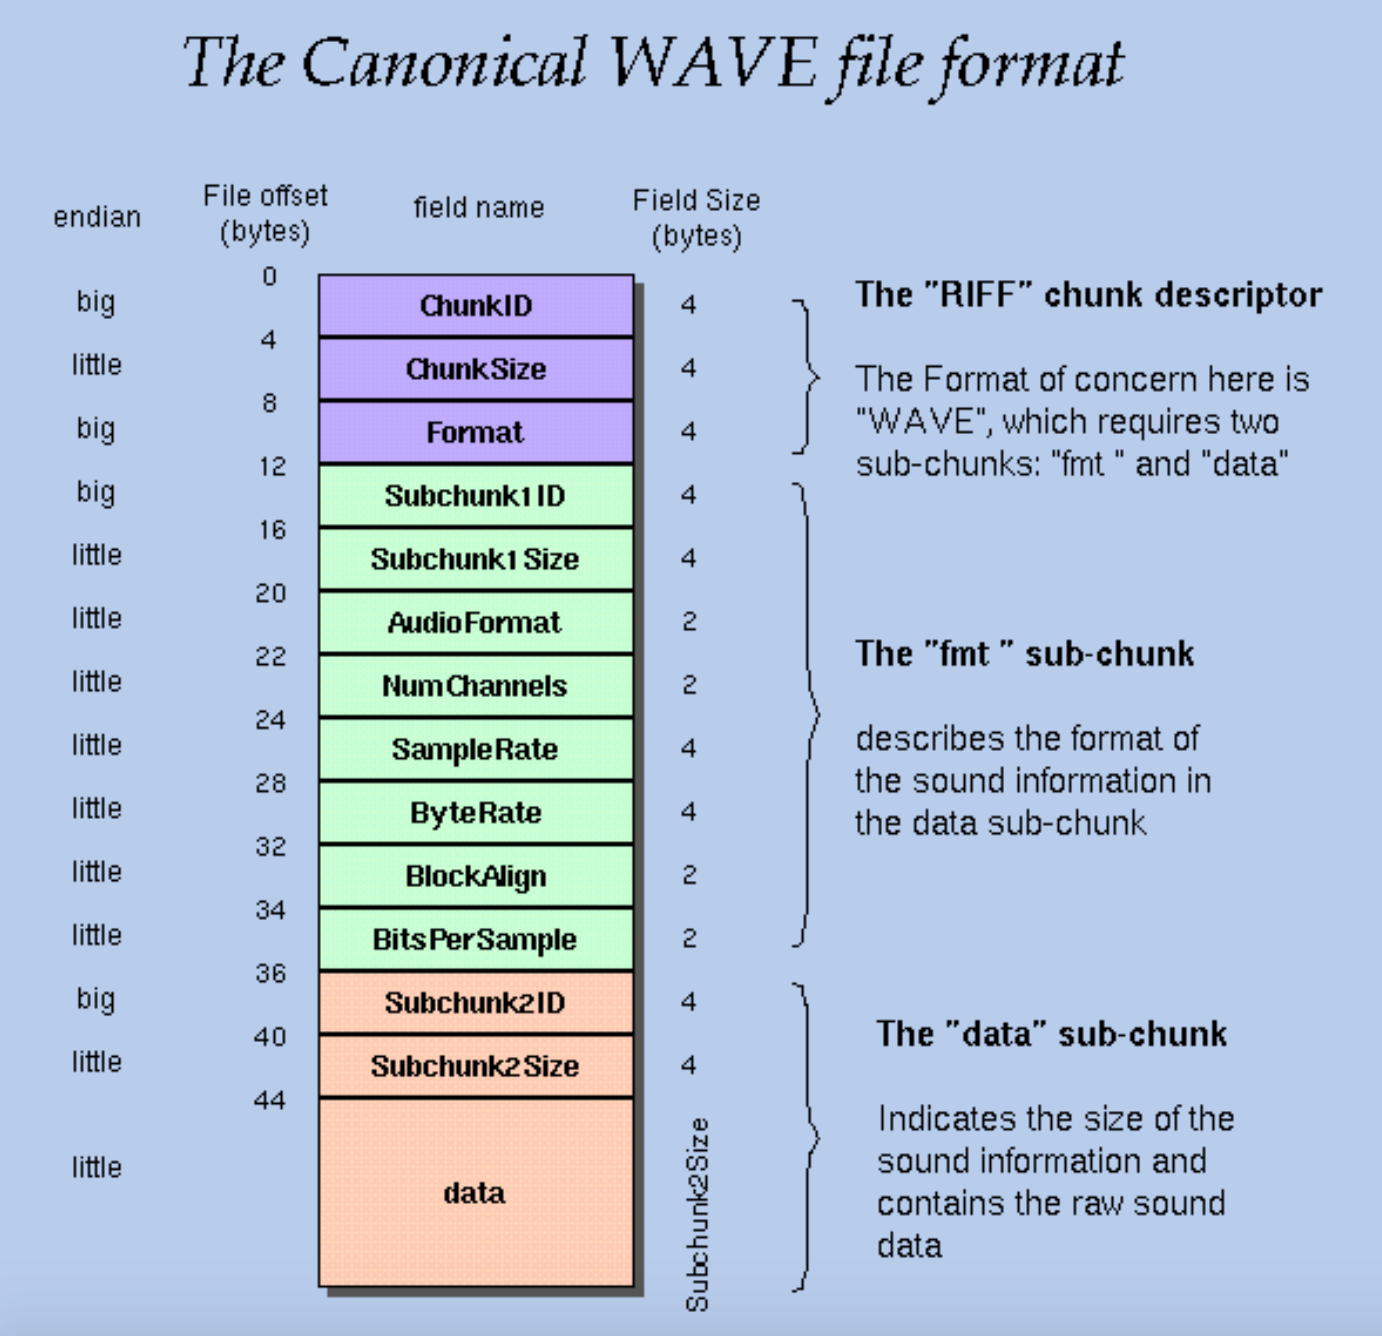
\includegraphics[width=9cm]{Figures/wave_format}
\decoRule
\caption[waveFormat]{Formato de archivos WAVE}
\label{fig:waveFormat}
\end{figure}

En resumen los ajustes que usaremos para capturar audio en formato WAV serán los siguientes:
\begin{itemize}
\item Codificación 16-bit PCM. 
\item Un solo canal o monocanal.
\item Frecuencia de muestreo: 44.1 kHz
\item Sistema \emph{little-endian} para almacenar los bytes.
\end{itemize}

En nuestro caso, hemos llevado a cabo esta captura de voz con la aplicación de captura y edición de audio Audacity \cite{REF} %REF a Audacity
, que es software libre y multiplataforma. En Audacity puedes especificar las configuraciones que indicamos en la descripción teórica que hemos presentado anteriormente; al leer un fichero raw será necesario indicar estos ajustes.

La forma de obtener el archivo de audio wav o raw es abierta. Usar Audacity es lo que nosotros hemos hecho pero se pueden obtener de muchas otras formas. Por ejemplo, un dato interesante es que todo dispositivo Android soporta la captura de audio con 1 canal a 44.1 kHz en codificación 16-bit PCM.\\

Ya tenemos hecho el primer paso, hemos conseguido los datos de audio en un formato que podemos manipular. El audio grabado está en bruto, lo siguiente será quitarle el ruido y frecuencias no útiles.

%----------------------------------------------------------------------------------------
%	SECTION 2
%----------------------------------------------------------------------------------------

\section{Filtrando el audio}

La segunda parte de nuestro procedimiento consiste en aplicar filtros para quedarnos con una versión más limpia de la voz que hemos grabado en el paso anterior. Como queremos que esta aplicación pueda adaptarse a varios interfaces de usuario (aplicaciones web, aplicaciones móviles y de escritorio) el sonido se podrá recoger de muchas maneras. Las frecuencias de voz que contienen información relevante están dentro de un rango relativamente estrecho y los micrófonos recogen un rango mayor. Por tanto cuando grabamos sonido, se recogen muchas frecuencias que no son útiles para el tratamiento de voz o speech. A través de un filtro pasabanda se podrán rechazar las frecuencias que se encuentran fuera del rango útil.

%-----------------------------------
%	SUBSECTION 2.1
%-----------------------------------
\subsection{Filtros}
 
Un filtro electrónico es cualquier medio que una señal atraviesa modificando la naturaleza de esta~\todo{referencia}. Los filtros son utilizados en el procesamiento de señales. Discriminan componentes de frecuencia de la señal, descartando o destacando las frecuencias requeridas pudiendo modificar la amplitud o la fase de la señal. \\%REF 

Un filtro puede ser analógico o digital. Nos centraremos en los filtros digitales porque estamos trabajando con una señal digital. 

%-----------------------------------
%	SUBSECTION 2.2
%-----------------------------------
\subsection{Filtros digitales}

Un filtro digital es un algoritmo que tiene como entrada un señal digital, es decir, una secuencia discreta de valores, y otra señal digital como salida. Se trata de operaciones matemáticas que alteran el espectro o el contenido frecuencial de la señal entrante, pudiendo modificar su amplitud o su fase. Se suelen utilizar para fortalecer o atenuar frecuencias, mejorar la calidad de la señal o para síntesis de sonido logrando efectos auditivos. \\%REF

En Procesamiento digital de señales (DSP por sus siglas en inglés) los filtros digitales se usan sobre los valores numéricos asociados a las muestras tomadas de señales analógicas. Siempre se puede hacer una conversión de señal analógica a digital y viceversa. Nosotros ya tenemos nuestra señal de audio en muestras y usaremos los filtros digitales. \\

Es interesante destacar que los filtros digitales muestran, en general, un mejor desempeño que los filtros analógicos, que operan con señales continuas y suelen consistir en un dispositivo hardware. Algunas de las ventajas de los filtros digitales sobre los analógicos son que los filtros digitales son programables y, por tanto, no tienen tantas restricciones como los segundos, se pueden conseguir características muy extremas e incluso hacer que se adapten a la señal según vaya siendo procesada. Son más fáciles de diseñar e implementar, y no les afectan las condiciones del ambiente.\\

Por estos motivos, entre otros, cuando se quiere filtrar una señal analógica y seguir obteniendo una señal analógica, se hace una conversión A/D tomando muestras de la señal analógica de entrada para obtener una señal digital (valores discretos). Después se le aplica un filtro digital para posteriormente hacer otra conversión D/A y volver a obtener una señal continua a partir de la señal digital ya filtrada. REF \\

En la figura \ref{fig:DSPanalog} se aprecia cómo se utilizan los filtros digitales para procesar señales analógicas con ayuda de conversores A/D (\emph{ADC}) y conversores D/A (\emph{DAC}).

\begin{figure}[th]
\centering
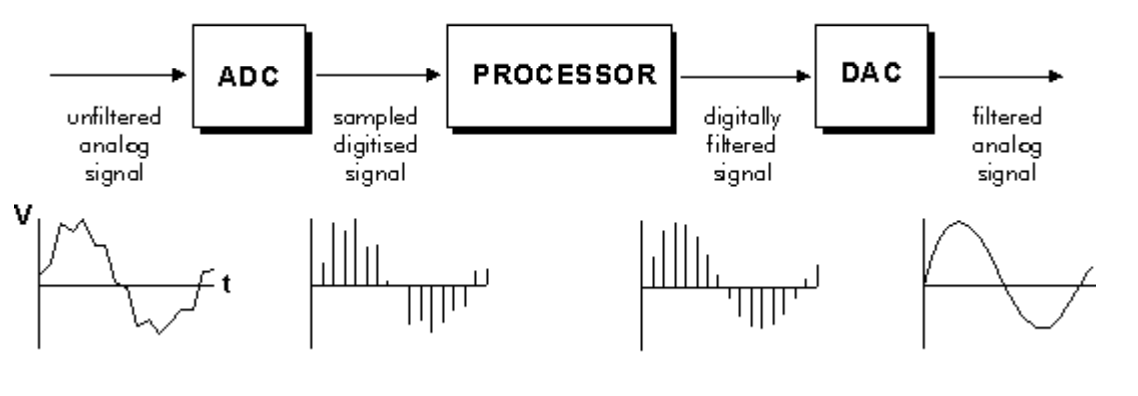
\includegraphics[width=10cm]{Figures/DSP-analog}
\decoRule
\caption[DSPanalog]{Proceso típico en DSP}
\label{fig:DSPanalog}
\end{figure}\todo{referencia}

Recordemos que nuestro objetivo principal es hacer a nuestra señal de audio comparable\todo{ser capaces de comparar dos señales de audio}. En esta fase inicial usaremos un filtro digital para quedarnos con un rango de frecuencias útiles. Las frecuencias que podemos percibir los humanos se encuentran entre 200 Hz y 20000 Hz. Y específicamente la voz humana se encuentra en un rango aún más pequeño como vimos en la sección anterior y puede observarse en la figura \ref{fig:limAudicion}.  

Los límites de la voz están entre 200-800 Hz y 3000-3500 Hz de frecuencia. Y serán valores como estos los que serán las frecuencias de corte en nuestro filtro.

%-----------------------------------
%	SUBSECTION 2.3
%-----------------------------------
\subsection{Tipos de filtros digitales}

Veremos a los filtros digitales como funciones que reciben una secuencia de números o valores (la señal de entrada) y produce una nueva secuencia de valores (la señal de salida filtrada).
Habrá varios tipos de filtros según el criterio que se escoja. Esta información nos ayudará a decidir qué filtros usaremos para nuestro propósito.

%-----------------------------------
%	SUBSUBSECTION 
%-----------------------------------
\subsubsection{Según la respuesta en frecuencia}

Es decir, de acuerdo a la parte del espectro que dejan pasar y que atenúan. De esta forma los filtros se puede seleccionar qué frecuencias quieren alterar y cuáles bloquear. Según esto podemos diferenciar 4 tipos básicos:

\begin{itemize}
\item \emph{Low-pass} o \emph{high-cut}. Deja pasar las frecuencias que están por debajo de una determinada frecuencia, por tanto, atenúa las frecuencia altas.
\item \emph{High-pass} o \emph{low-cut}. Deja pasar las frecuencias que están por encima de una determinada frecuencia, por tanto, para las frecuencia bajas.
\item \emph{Band-pass}. El filtro pasabanda es la combinación de un filtro low-pass y uno high-pass, este filtro deja pasar las frecuencias que están en una determinada banda de frecuencia, es decir, entre dos frecuencias determinadas.
\item \emph{Band-stop} o \emph{band-reject}. También es combinación de un filtro low-pass y otro high-pass, pero este deja pasar la mayor parte de las frecuencias sin alterar y atenúa las de un rango especificado, es decir, bloquea las frecuencias de la banda determinada por dos frecuencias.
\end{itemize}

Los dos primeros tipos se definen por su frecuencia de corte. Y los dos últimos tipos de filtros se definen por su frecuencia central y su ancho de banda.\\

La frecuencia de corte es aquella se encuentra en el límite entre la banda pasante y la atenuada. Las frecuencias bien por encima o por debajo de ella se ven atenuadas por un factor de $1/ \sqrt{2}$ (aproximadamente 0.707). 

Llamamos banda pasante (\emph{passband}) al rango de frecuencias que no se verán afectadas por el filtro y simplemente pasarán. Mientras que la banda atenuada (\emph{stopband}) son aquellas frecuencias que el filtro bloquea. Las transiciones entre la banda pasante y la banda de corte no son generalmente limpias en los filtros reales. Existe, por tanto, una banda de transición.

%-----------------------------------
%	SUBSUBSECTION 
%-----------------------------------
\subsubsection{Expresión general de un filtro y clasificación por respuesta al impulso}

Podemos ver la ecuación de un filtro  en función del número de muestras (n):
$$y(n)= {\sum_{k=0}^N} b_k \cdot x(n-k) - {\sum_{k=1}^M} a_k \cdot y(n-k)$$ \label{eq:filterEq} \todo{poner etiquetas visibles a las ecuaciones}

El filtro se ve definido por la elección de los coeficientes $a$ y $b$. Y depende tanto de las muestras de entrada anteriores como de las muestras ya filtradas. El número de muestras anteriores que el filtro utiliza y mezcla con la nueva muestra de entrada nos da el orden del filtro. \\

Si la salida $y(n)$  solo se calcula con las muestras de entrada se dice que el filtro definido es no-recursivo. Por otro lado, un filtro recursivo es aquel que también utiliza los valores de salida calculados antes.

Estos dos filtros también son conocidos como FIR (Respuesta finita al impulso o \emph{Finite Impulse Response}) e IIR (Respuesta infinita al impulso o \emph{Infinite Impulse Response}), respectivamente.
Estos términos son la clasificación de los filtros según su respuesta al impulso. La respuesta al impulso de un filtro digital es la secuencia de salida cuando el filtro tiene como entrada la señal impulso o entrada unitaria, siendo un esta una muestra con el valor 1 seguida de más muestras pero con valor cero. \cite{ref1} %%%REF: http://www.atmel.com/Images/doc2527.pdf

%----------------------------------
\paragraph{Filtros FIR}

Los filtros FIR cuando tienen como entrada la señal impulso producen como salida un número finito de términos. Para obtener las salidas $y(n)$ se retrasa la señal de entrada hasta ese momento y se combina con la nueva señal de entrada $x(n)$. Se trata de un combinación lineal y solo están implicadas señales de la entrada, tanto la presente como las pasadas.
Si vemos la ecuación anterior, para los filtros FIR queda de la siguiente forma

$$ y[n] = b_0 \cdot x[n] + b_1 \cdot x[n - 1] + b_2 \cdot x[n - 2] + \cdots + b_N \cdot x[n - N] $$

Solo están presentes los coeficientes $b_i$ que determinan el comportamiento del filtro. Se tienen $N+1$ coeficientes y $N$ es el orden filtro. De hecho, la respuesta del filtro FIR a la señal impulso 
$$ x = \{1, 0, 0, 0, 0, 0, 0, \ldots \} $$
es la señal
$$ y = \{b_0, b_1, b_2, b_3, \ldots, b_N , 0, 0, 0, \ldots \}  $$
donde se pueden ver los coeficientes y la finitud.

%----------------------------------
\paragraph{Filtros IIR}

Los filtros IIR producen una salida infinita, esto se produce por la recursión en su ecuación. Ya que tanto a como b son no nulos y la ecuación siempre es de la forma
$$y[n] = b_0 \cdot x[n] + b_1 \cdot x[n - 1] + b_2 \cdot x[n - 2] + \cdots + b_N \cdot x[n - N]  $$
$$- a_1 \cdot y[n - 1] - a_2 \cdot y[n - 2] - a_3 \cdot y[n - 3] - \cdots - a_M \cdot y[n - M] $$
\label{eq:filterEqIIR}

Es decir, para la respuesta $y[n]$ se tiene una combinación lineal de entradas hasta ese momento, la señal de entrada actual y señales de salida anteriores. Se tienen $N+1$ términos del coeficiente $b$ y $M$ términos del coeficiente a. El orden de un filtro IIR es el máximo entre $N$ y $M$.

Se dice que se retroalimenta, por eso son también llamados recursivos o de feedback. Y por ese motivo se dice que su respuesta es teóricamente infinita, siempre habrá términos de salida que sirvan entrada en la fórmula. Pero en realidad, a términos prácticos, la respuesta de casi todos los filtros IIR se reduce a cero en tiempo finito.

%----------------------------------
\paragraph{FIR vs IIR. Función de transferencia}

La función de transferencia de ambos filtros se calcula con el uso de la transformada Z sobre la respuesta al impulso. Lo que teníamos, una función cuyo dominio discreto es el tiempo, con la aplicación de esta transformación, ahora es una función con dominio la frecuencia y cuya variable es compleja. De esta manera, vemos la respuesta en impulso como respuesta en frecuencia. Esta forma de representar los filtros nos da información sobre los ceros y polos de la ecuación del filtro. 

$$ H(z)={\frac {B(z)}{A(z)}}={\frac  {{b_{{0}}+b_{{1}}z^{{-1}}+b_{{2}}z^{{-2}}+\cdots +b_{{N}}z^{{-N}}}}{{1+a_{{1}}z^{{-1}}+a_{{2}}z^{{-2}}+\cdots +a_{{M}}z^{{-M}}}}} $$
\label{eq:filterEqFIR}

Los filtros IIR y FIR se distinguen en los siguientes elementos:
\begin{itemize}
\item Tiempo de cómputo. Mirando las ecuaciones \ref{eq:filterEqIIR} y \ref{eq:filterEqFIR} %FIX referencias a ecuaciones
parece que los filtros IIR o recursivos requieren realizar más cálculos ya que dependen tanto de términos de la señal de entrada como de términos ya calculados de la salida. Pero, en general, ocurre lo contrario. Para conseguir la respuesta según unas ciertas especificaciones, los filtros IIR necesitan un menor número de coeficientes que los filtros FIR. Es decir, el filtro IIR requiere un orden menor para conseguir las especificaciones, haciendo que el cómputo sea más rápido, la memoria requerida, el número de operaciones y el tiempo de cómputo es menor.
\item Estabilidad. Si vemos la función de transferencia de ambos filtros se ve que un filtro IIR puede tener polos y por tanto, inestabilidad, mientras que un FIR sólo tiene ceros, y por eso, siempre es estable y no entra en oscilación
\item Respuesta de fase lineal. La fase es la relación que se hay entre un punto de la señal de entrada y su imagen por el filtro. La fase es así una función que idealmente es lineal. Pero esta linealidad solo se consigue realmente con los filtros FIR. La respuesta de fase de los filtros IIR no es lineal, sobre todo cerca a la banda de transición, pero se pueden hacer buenas aproximaciones. Además, si estas bandas de transición son muy cortas, es decir se hacen cortes muy abruptos, los FIR pueden requerir un gran número de retardos. Mientras que los IIR pueden ofrecer cortes muy marcados. 
\end{itemize}

Estas son las diferencias más notables, pero con la tecnología actual la diferencia entre los dos tipos es poco perceptible.


%-----------------------------------
%	SUBSUBSECTION 
%-----------------------------------
\subsubsection{Los filtros que usaremos} %parece que son varios epro solo es uno

Sabemos que los filtros \emph{bandpass} se pueden construir a partir de los \emph{lowpass}. Lo que queremos es desechar las frecuencias que se salen del rango especificado y por eso usaremos un \emph{bandpass}. Habrá cortes que atenúen frecuencias muy bajas y muy altas. El filtro lowpass que usaremos como base para el bandpass debe intentar hacer un corte limpio. Este filtro electrónico ideal del que hablamos es el llamado filtro \emph{brick-wall}, el cual deja pasar por completo la banda de paso y atenúa el resto con una transición muy abrupta. El nombre se debe a la forma que tiene su función de transferencia: constante hasta que se llega a la frecuencia de corte donde la intensidad de la señal tiende a menos infinito casi de inmediato. 

\begin{figure}[th]
\centering
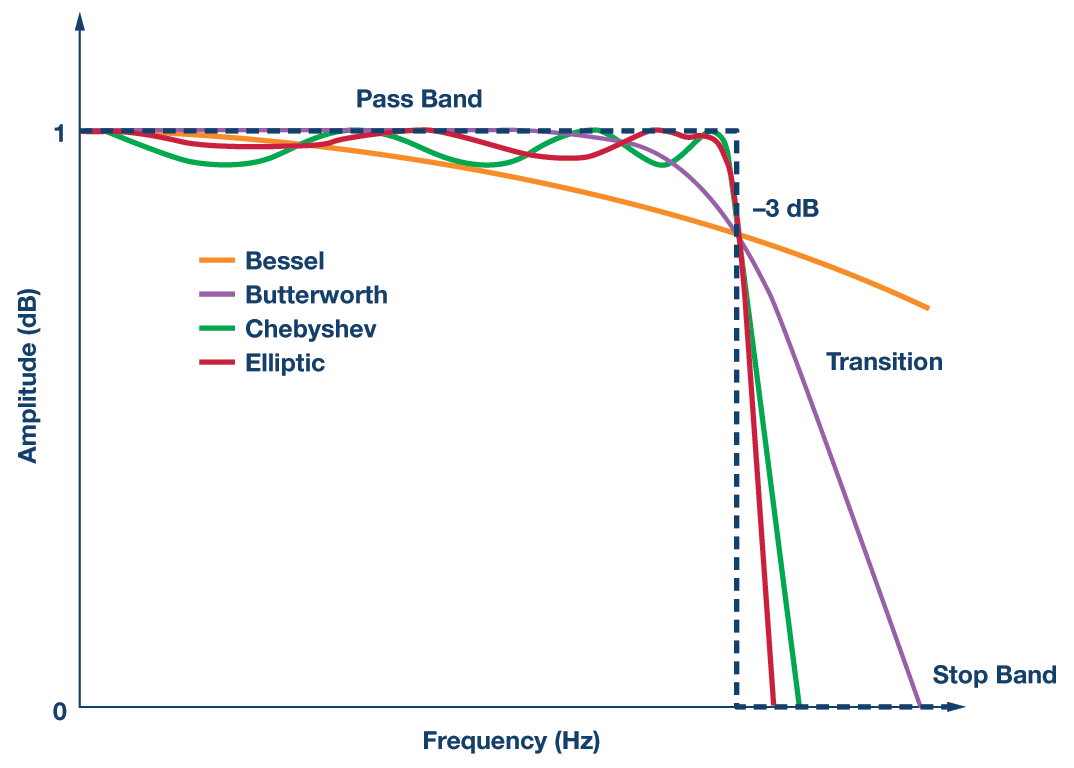
\includegraphics[width=9cm]{Figures/4filters}
\decoRule
\caption[4filters]{Diagramas de Bode a partir de la función de transferencia de los filtros Bessel, Butterworth, Chebyshev y elíptico}
\label{fig:4filters}
\end{figure}

Los filtros electrónicos cuyo comportamiento más se asemejan a este filtro ideal son Butterworth, Chebyshev I, Chebyshev II, elíptico, y Bessel. Estos son la versión digital de sus homónimos analógicos.

Casi todos los filtros analógicos son IIR, sin embargo los filtros digitales pueden ser FIR o IIR. Recordamos que la presencia de la retroalimentación en el filtro hace que este sea IIR. \\

Entre las opciones que tenemos elegimos usar el filtro Butterworth, que va a preservar la parte de la señal que queremos.

%-----------------------------------
%	SUBSECTION 2.4
%-----------------------------------
\subsection{IMPLEMENTACIÓN}

Programar un filtro conlleva dos pasos. Primero, teniendo claro que nuestro filtro digital es IIR, sabemos que debemos conseguir los coeficiente $a$ y $b$ que definirán a nuestro filtro. Y segundo, una vez tenemos los coeficientes podemos aplicarlos a cualquier entrada que le demos a nuestro filtro y obtendremos la señal filtrada.\\

Para obtener los coeficientes que definen al filtro lo que hicimos fue documentarnos sobre cómo lo implementan en bibliotecas de lenguajes como Python y Matlab. 
Al principio se intentó aprovechar que Python tiene métodos específicos para el filtrado de señales pero como en esos momentos se intentaba hacer una aplicación android en Android Studio, trabajar desde ese entorno con Python no resultó muy fructuoso. Se estudiaron Jython y SL4A (\emph{Script Layer for Android})\todo{referencias} como posibles puentes. Pero resultaron un poco complicados para alguien que no tiene experiencia en Android. Como la final se optó por una aplicación Java se implementó el cálculo de los coeficientes y el filtrado en una clase de Java. \\

Para calcular ambos coeficientes se necesita usar números complejos así que se añadió la biblioteca \code{commons-math3-3.6.1}\todo{referencia} y se utilizó en concreto la clase \\\code{org.apache.commons.math3.complex.Complex}. Por otro lado, ambos coeficientes dependen tanto de la frecuencia de muestreo $f_s$, las frecuencias de corte y del orden del filtro. Estos datos serán parámetros que se especifican al crear el filtro. Estamos creando un filtro pasabanda entonces habrán dos cortes. 

Cuando le pasemos estos parámetros a nuestro constructor del filtro, hay que hacer un pequeño preprocesamiento. Lo que se quiere es tener en cuenta el Teorema de muestreo de Nyquist-Shannon y hacer que los cortes estén entre 0 y 1. Lo que haremos es usar la mitad de $f_s$ como el máximo de las frecuencias captadas $f_m$ según el teorema mencionado y después calcular las razones de los cortes, es decir la frecuencia de corte dividido entre $f_m$.

El orden del filtro condicionará el número de términos que tendrán $a$ y $b$. Para conseguir un filtro Butterworth se realizan una serie de operaciones que pueden ser consultadas en el código fuente de de ese método en Pyhton \cite{REF} % https://github.com/scipy/scipy/blob/v0.18.1/scipy/signal/filter_design.py#L1861-L1932
, obtendremos $2*N+1$ términos para $a$ y $b$ siendo $N$ el orden del filtro.

Una vez que tenemos los coeficientes calculados ya podemos aplicar la ecuación~\ref{eq:filterEq} para conseguir la salida $y$. De esta manera obtenemos nuestra señal filtrada.




 
%\include{Chapters/Chapter3}
%\include{Chapters/Chapter4} 
%\include{Chapters/Chapter5} 

%----------------------------------------------------------------------------------------
%	THESIS CONTENT - APPENDICES
%----------------------------------------------------------------------------------------

\appendix % Cue to tell LaTeX that the following "chapters" are Appendices

% Include the appendices of the thesis as separate files from the Appendices folder
% Uncomment the lines as you write the Appendices

% Appendix A

\chapter{Frequently Asked Questions} % Main appendix title

\label{AppendixA} % For referencing this appendix elsewhere, use \ref{AppendixA}

\section{How do I change the colors of links?}

The color of links can be changed to your liking using:

{\small\verb!\hypersetup{urlcolor=red}!}, or

{\small\verb!\hypersetup{citecolor=green}!}, or

{\small\verb!\hypersetup{allcolor=blue}!}.

\noindent If you want to completely hide the links, you can use:

{\small\verb!\hypersetup{allcolors=.}!}, or even better: 

{\small\verb!\hypersetup{hidelinks}!}.

\noindent If you want to have obvious links in the PDF but not the printed text, use:

{\small\verb!\hypersetup{colorlinks=false}!}.
%%%
The color of links can be changed to your liking using:

{\small\verb!\hypersetup{urlcolor=red}!}, or

{\small\verb!\hypersetup{citecolor=green}!}, or

{\small\verb!\hypersetup{allcolor=blue}!}.

\noindent If you want to completely hide the links, you can use:

{\small\verb!\hypersetup{allcolors=.}!}, or even better: 

{\small\verb!\hypersetup{hidelinks}!}.

\noindent If you want to have obvious links in the PDF but not the printed text, use:

{\small\verb!\hypersetup{colorlinks=false}!}.
%%%
The color of links can be changed to your liking using:

{\small\verb!\hypersetup{urlcolor=red}!}, or

{\small\verb!\hypersetup{citecolor=green}!}, or

{\small\verb!\hypersetup{allcolor=blue}!}.

\noindent If you want to completely hide the links, you can use:

{\small\verb!\hypersetup{allcolors=.}!}, or even better: 

{\small\verb!\hypersetup{hidelinks}!}.

\noindent If you want to have obvious links in the PDF but not the printed text, use:

{\small\verb!\hypersetup{colorlinks=false}!}.
%%%
The color of links can be changed to your liking using:

{\small\verb!\hypersetup{urlcolor=red}!}, or

{\small\verb!\hypersetup{citecolor=green}!}, or

{\small\verb!\hypersetup{allcolor=blue}!}.

\noindent If you want to completely hide the links, you can use:

{\small\verb!\hypersetup{allcolors=.}!}, or even better: 

{\small\verb!\hypersetup{hidelinks}!}.

\noindent If you want to have obvious links in the PDF but not the printed text, use:

{\small\verb!\hypersetup{colorlinks=false}!}.
%%%
The color of links can be changed to your liking using:

{\small\verb!\hypersetup{urlcolor=red}!}, or

{\small\verb!\hypersetup{citecolor=green}!}, or

{\small\verb!\hypersetup{allcolor=blue}!}.

\noindent If you want to completely hide the links, you can use:

{\small\verb!\hypersetup{allcolors=.}!}, or even better: 

{\small\verb!\hypersetup{hidelinks}!}.

\noindent If you want to have obvious links in the PDF but not the printed text, use:

{\small\verb!\hypersetup{colorlinks=false}!}.
%%%
The color of links can be changed to your liking using:

{\small\verb!\hypersetup{urlcolor=red}!}, or

{\small\verb!\hypersetup{citecolor=green}!}, or

{\small\verb!\hypersetup{allcolor=blue}!}.

\noindent If you want to completely hide the links, you can use:

{\small\verb!\hypersetup{allcolors=.}!}, or even better: 

{\small\verb!\hypersetup{hidelinks}!}.

\noindent If you want to have obvious links in the PDF but not the printed text, use:

{\small\verb!\hypersetup{colorlinks=false}!}.
%%%
%\include{Appendices/AppendixB}
%\include{Appendices/AppendixC}

%----------------------------------------------------------------------------------------
%	BIBLIOGRAPHY
%----------------------------------------------------------------------------------------

\renewcommand{\bibname}{Bibliografía}             %Bibliography REferencias refname
 \renewcommand{\refname}{Bibliografía}             %Bibliography REferencias refname
 
\begin{thebibliography}{9}

\bibitem{REF}
  poner referencia %%%%%%%%%% ! ! ! ! ! ! ! !  %%%%%
  
\bibitem{lamport94}
  Leslie Lamport,
  \emph{\LaTeX: a document preparation system},
  Addison Wesley, Massachusetts,
  2nd edition,
  1994.
  
  

\end{thebibliography}
\printbibliography[heading=bibintoc]

%----------------------------------------------------------------------------------------

\end{document}  
